\documentclass[fontsize=11pt,reqno,a4paper,oneside]{scrartcl}

% ---- Sprache und Textformatierung ----
\usepackage{fontspec}
\usepackage{polyglossia}
\setdefaultlanguage{english}
\usepackage{microtype}
\usepackage{csquotes}
\usepackage{acronym}

% ---- KOMA-Script Seiteneinstellungen ----
\usepackage[onehalfspacing]{setspace}  
\usepackage[headsepline]{scrlayer-scrpage}

% Kopfzeilen-Konfiguration
\clearpairofpagestyles  % Alle bestehenden Kopf- und Fußzeilen löschen
\addtokomafont{pagehead}{\normalfont\small}  % Schriftart der Kopfzeile
\automark[section]{section}
\ihead{\textsc{\headmark}} 
\cfoot{\pagemark}

% ---- Mathematik und Symbole ----
\usepackage{amsmath, amsthm, amssymb, mathtools}
\usepackage[version=4]{mhchem}
\usepackage{chemformula}
\newcommand{\angstrom}{\text{\normalfont\AA}}

% ---- Graphische Pakete ----
\usepackage{xcolor}
\usepackage{graphicx}
\usepackage{float}
\usepackage{siunitx}
\usepackage{textpos}
\usepackage{subfig}
\usepackage{svg}

% ---- Text-Positionierung ----
\usepackage[pscoord]{eso-pic}
\newcommand{\placetextbox}[3]{% \placetextbox{<horizontal pos>}{<vertical pos>}{<stuff>}
  \setbox0=\hbox{#3}% Put <stuff> in a box
  \AddToShipoutPictureFG*{% Add <stuff> to current page foreground
    \put(\LenToUnit{#1\paperwidth},\LenToUnit{#2\paperheight}){\vtop{{\null}\makebox[0pt][c]{#3}}}%
  }%
}%

% ---- Bibliographie ----
\usepackage[backend=biber,
    citestyle=numeric-comp,
    bibstyle=numeric,
    bibwarn=true,
    autocite=superscript,
    abbreviate=true, 
    sorting=none, 
    url=false, 
    doi=false,
    eprint=false,
    isbn=false]{biblatex}

% Definition eines neuen Zitierbefehls mit eckigen Klammern
\DeclareCiteCommand{\supercite}[\mkbibsuperscript]%
    {\usebibmacro{cite:init}%
        \let\multicitedelim\supercitedelim%
        \iffieldundef{prenote}%
        {}%
        {\BibliographyWarning{Ignoring prenote argument}}%
        \iffieldundef{postnote}%
        {}%
        {\BibliographyWarning{Ignoring postnote argument}}%
        \bibleftbracket}%
    {\usebibmacro{citeindex}%
        \usebibmacro{cite:comp}}
    {}%
    {\usebibmacro{cite:dump}%
        \bibrightbracket}

% Bibliographie-Dateien
\addbibresource{/Users/lucashirschfeld/sciebo/VsCode/LaTeX-Projects/bibliography/zotero.bib}

% ---- Hyperlinks ----
\usepackage{hyperref}
\hypersetup{colorlinks=true, linkcolor=black, citecolor=black, urlcolor=black}

% ---- Dokumenteinstellungen ----
\setlength{\parindent}{0pt}

% ---- Metadaten ----
\def\Autor{Lucas Hirschfeld, s6luhirs@uni-bonn.de}
\def\Titel{Low Energy Electron Diffraction (\ac{LEED})}
\def\Date{First Submission: \today}
\def\PiC{Supervisor: Morris Mühlpointner}
\def\Abstract{Low Energy Electron Diffraction (\ac{LEED}) is a powerful technique for the structural analysis of crystalline surfaces. This report explores the principles, experimental setup, and applications of \ac{LEED} in surface science.} 

\begin{document}
\pagestyle{empty}
\begin{titlepage}
    \begin{center}
        \vspace*{\fill}
        {\LARGE\bfseries \Titel}\par\vspace{2cm}
        {\Autor\par\vspace{0.5cm}\PiC\par\vspace{1cm}\par\vspace{0.2cm}\Date\par\vspace{5cm}}
    \end{center}
    {\Abstract\vspace{0.5cm}\par}\vfill
\end{titlepage}

\pagestyle{scrheadings}
\tableofcontents
\pagenumbering{arabic}
\clearpage

\section{Introduction}

\ac{LEED} has established itself as one of the most powerful and widely used techniques for determining the surface structure of crystalline materials\supercite{VanHove1986}. The technique exploits the wave nature of electrons, first proposed by de Broglie in 1924, utilizing electrons with energies typically between 20-200 eV. At these energies, electrons possess wavelengths comparable to interatomic distances (0.1-0.3 nm) while exhibiting limited penetration depths of only a few atomic layers\supercite{Woodruff2016}.

The historical significance of \ac{LEED} extends back to 1927 when Davisson and Germer first observed electron diffraction from a nickel surface, providing experimental confirmation of de Broglie's matter wave hypothesis\supercite{Davisson1927}. However, it was not until the 1960s that \ac{LEED} evolved into a reliable analytical technique, coinciding with advancements in ultra-high vacuum technology and computational methods\supercite{Pendry1990}.

The fundamental principle of \ac{LEED} relies on elastic scattering of low-energy electrons from a periodic crystal surface. The resulting diffraction pattern directly reflects the reciprocal lattice of the surface structure, allowing determination of the surface symmetry, lattice parameters, and reconstruction phenomena\supercite{Ertl}. In contrast to X-ray diffraction techniques that probe bulk properties, \ac{LEED}'s surface sensitivity arises from the limited mean free path of low-energy electrons in solid materials, making it uniquely suited for surface crystallography\supercite{Seah1979}.

Modern \ac{LEED} analysis extends beyond qualitative pattern interpretation to include quantitative structural determinations. By systematically measuring diffraction spot intensities as a function of electron energy (I-V curves) and comparing them with theoretical calculations, atomic positions within the surface unit cell can be determined with precision approaching 0.01 nm. This approach has been crucial in elucidating complex surface reconstructions, adsorbate structures, and the atomic mechanisms underlying surface phenomena\supercite{Heinz1995}.

The integration of \ac{LEED} with complementary techniques such as \ac{STM}, \ac{XPS}, and \ac{AES} has created powerful methodological combinations for comprehensive surface characterization\supercite{Fadley2010}. Furthermore, recent innovations including \ac{SPA-LEED} and \ac{LEEM} have extended the capabilities to include analysis of surface defects, domain sizes, and dynamic processes\supercite{Henzler1991}.

This report explores the experimental foundations, working principles, and practical applications of \ac{LEED} in surface science. Particular emphasis is placed on the interpretation of diffraction patterns, quantitative analysis methodologies, and case studies demonstrating \ac{LEED}'s role in solving significant surface structural problems in heterogeneous catalysis, thin film growth, and materials science.

\clearpage
\section{Experimental}

% Hier Ihren Text für den Experimental-Teil einfügen

\subsection{Sample Preparation}

The Au(111) single crystal surface was prepared following standard ultra-high vacuum (UHV) procedures. The sample was mounted in the UHV chamber and subjected to repeated cleaning cycles consisting of Ar$^+$ ion sputtering at 1 keV for 10 minutes followed by annealing at 750 K for 15 minutes. This cleaning procedure was repeated until a sharp $(1 \times 1)$ LEED pattern characteristic of the clean Au(111) surface was observed, indicating removal of surface contaminants and achievement of a well-ordered surface structure.

\subsection{LEED Measurements}

Low Energy Electron Diffraction measurements were performed using a standard reverse-view LEED system equipped with a hemispherical fluorescent screen and CCD camera. The electron gun was operated at various energies between 50-200 eV with a beam current of approximately 1-5 $\mu$A to minimize beam damage while maintaining sufficient signal intensity.

The experimental procedure consisted of:

1. Initial verification of surface cleanliness through observation of the characteristic Au(111)-$(1 \times 1)$ diffraction pattern
2. Systematic energy variation from 50-200 eV in 2-5 eV increments
3. Recording of LEED patterns at each energy step using the camera system
4. Measurement of diffraction spot intensities for generation of I-V curves

Key diffraction beams monitored included the (00), (10), and (11) spots along with their symmetry equivalents. The sample was maintained at room temperature throughout the measurements under UHV conditions with base pressure below $5 \times 10^{-10}$ mbar.

\subsection{Data Analysis}

The recorded LEED images were analyzed using appropriate software to extract quantitative intensity-voltage (I-V) curves. Background subtraction was performed to account for inelastic scattering contributions, and spot intensities were normalized to compensate for variations in beam current and overall intensity fluctuations between different energy measurements.

\clearpage
\section{Results}

\clearpage
\section{Results}

\subsection{Orientation of the surface}

\begin{figure}[H]
    \centering
    \subfloat[\ac{LEED} orientation]{
        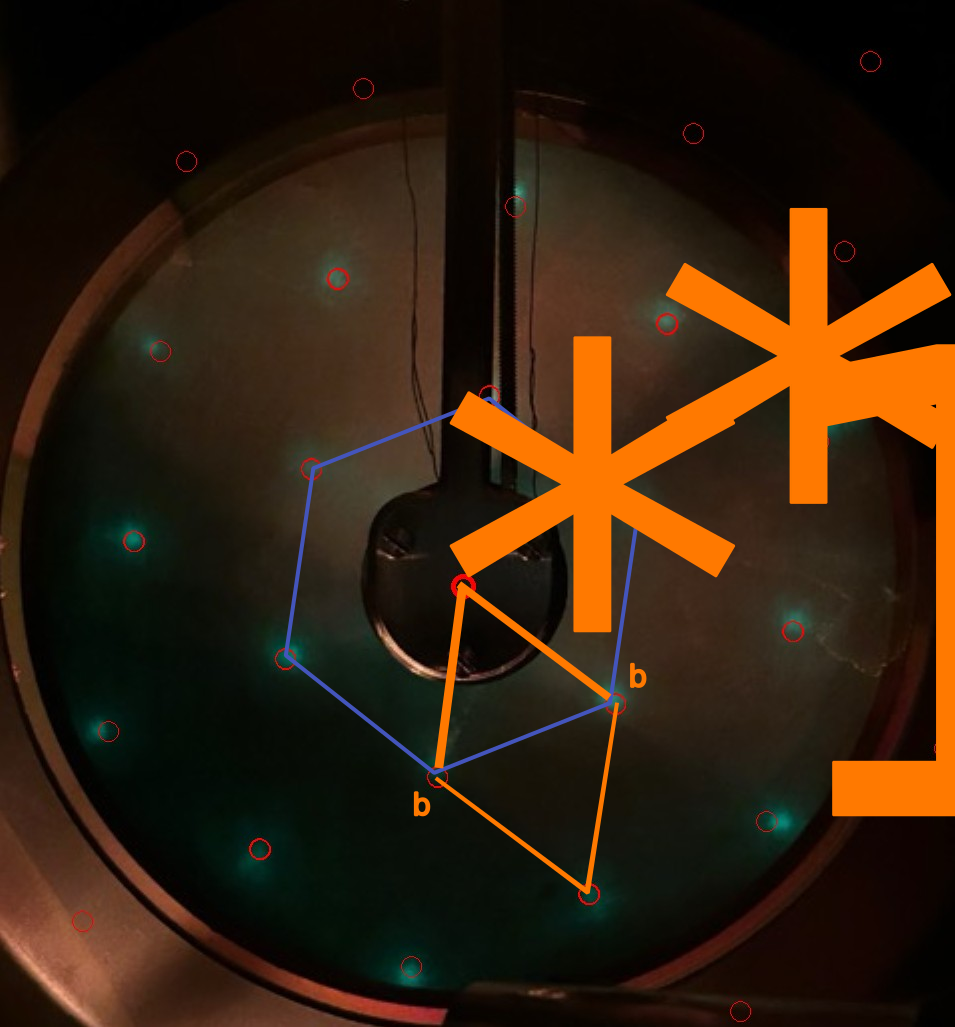
\includegraphics[width=0.47\textwidth]{images/image1-2.png}
        \label{fig:leed_orientation}
    }
    \hfill
    \subfloat[Crystal orientation]{
        \includegraphics[width=0.47\textwidth]{images/surface-2.png}
        \label{fig:crystal_orientation}
    }
    
    \caption{Surface orientation for Au(111) crystal structure.}
    \label{fig:surface_orientations}
\end{figure}

\subsection{Determination of the spot distances}
The \ac{LEED} measurements of the Au(111) surface revealed a well-ordered $(1 \times 1)$ diffraction pattern characteristic of the clean, reconstructed surface. \autoref{fig:leed_patterns} shows the evolution of the diffraction pattern at different electron energies, demonstrating the energy-dependent intensity variations of the diffraction spots.

\begin{figure}[H]
    \centering
    \subfloat[0° rotation]{
        \includegraphics[width=0.47\textwidth]{images/119.6eV-1428-1054-1091-1310-1187-1219.jpg}
        \label{fig:leed_0deg}
    }
    \hfill
    \subfloat[5° rotation]{
        \includegraphics[width=0.47\textwidth]{images/119.6ev-1428-1073-1094-1310-1197-1251-283Grad-1.jpg}
        \label{fig:leed_5deg}
    }
    
    \vspace{0.5cm}
    
    \subfloat[10° rotation]{
        \includegraphics[width=0.47\textwidth]{images/119.6eV-1428-1073-1094-1310-1197-1251-288Grad.jpg}
        \label{fig:leed_10deg}
    }
    \hfill
    \subfloat[15° rotation]{
        \includegraphics[width=0.47\textwidth]{images/120.5eV-1442-1085-1109-1326-1208-1262-293Grad.jpg}
        \label{fig:leed_15deg}
    }
    
    \caption{LEED patterns of Au(111) surface at an electron energy of 119.6~\si{eV} showing the characteristic diffraction pattern. The red circles indicate the positions of the diffraction spots.}
    \label{fig:leed_patterns}
\end{figure}

The diffraction patterns clearly show the hexagonal symmetry expected for the Au(111) surface. The (00) spot at the center corresponds to the specularly reflected beam, while the surrounding first-order spots (10), (01), and (11) along with their symmetry equivalents form the characteristic hexagonal pattern. The intensity of these spots varies systematically with electron energy, providing the basis for quantitative I-V curve analysis.

The spot positions remain constant across all energies, confirming the absence of surface reconstruction and the maintenance of the bulk-terminated $(1 \times 1)$ structure. The background intensity and overall pattern quality indicate a well-ordered surface with low defect density, validating the effectiveness of the cleaning procedure described in the experimental section.

\subsection{Determination of the lattice constant of the Au(111) surface}

\begin{figure}[H]
    \centering
    \subfloat[80.0 eV]{
        \includegraphics[width=0.47\textwidth]{images/80.0eV-858-719-828-831-718-490.jpg}
        \label{fig:leed_80eV}
    }
    \hfill
    \subfloat[120.0 eV]{
        \includegraphics[width=0.47\textwidth]{images/120.0eV-1435-1156-1080-1321-1201-1010.jpg}
        \label{fig:leed_120eV}
    }
    
    \vspace{0.5cm}
    
    \subfloat[179.3 eV]{
        \includegraphics[width=0.47\textwidth]{images/179.3eV-2005-1740-2255-1883-1692-1849.jpg}
        \label{fig:leed_179eV}
    }
    \hfill
    \subfloat[198.7 eV]{
        \includegraphics[width=0.47\textwidth]{images/198.7eV-2209-1887-2196-2268-1912-1786.jpg}
        \label{fig:leed_198eV}
    }
    
    \caption{LEED patterns of Au(111) surface at different electron energies showing the characteristic diffraction pattern. The red circles indicate the positions of the diffraction spots.}
    \label{fig:leed_patterns_energy}
\end{figure}

\subsection{The reconstruction of the Au(111) surface}

\begin{figure}[H]
    \centering
    \subfloat[23.6~\si{eV}]{
        \includegraphics[width=0.47\textwidth]{images/(R-23.6eV-320-204-334331-243-153-((11,0),(0.5,1.0)).jpg}
        \label{fig:reconstruction_23.4eV}
    }
    \hfill
    \subfloat[67.4~\si{eV}]{
        \includegraphics[width=0.47\textwidth]{images/R-67.4eV-821-646-846-927-691-417-((11,0),(0.5,1)).jpg}
        \label{fig:reconstruction_67.4eV}
    }

    \caption{\ac{LEED} patterns of the Au(111) surface at two different electron energies with the sample rotated showing the characteristic Au(111) reconstruction. The blue circles indicate the positions of the substrate spots. The reconstruction is indicated by the additional red circles in the pattern.}
    \label{fig:reconstruction}
\end{figure}

\subsection{PTCDA on the Au(111) surface by epitaxial growth}

\begin{figure}
    \centering
    \includegraphics[width=0.47\textwidth]{images/23.4eV-327-329-311-316-233-231-2-((-0.92,4.66),(-7.87,-2.93)).jpg}
    \caption{\ac{LEED} pattern of \ac{PTCDA} on the Au(111) surface at an electron energy of 23.4~\si{eV}. The red circles indicate the positions of the center and the purple spots indicates the diffraction spots of the superstructure.}
    \label{fig:ptcda}
\end{figure}

\clearpage
\section{Discussion}
% Hier Ihren Text für den Discussion-Teil einfügen

\clearpage
\section{Appendix}

\subsection*{Acronyms}

\begin{acronym}
    \acro{LEED}{low energy electron diffraction}
    \acro{LEEM}{low energy electron microscopy}
    \acro{STM}{scanning tunneling microscopy}
    \acro{XPS}{x-ray photoelectron spectroscopy}
    \acro{AES}{auger electron spectroscopy}
    \acro{SPA-LEED}{spot-profile analysis low energy electron diffraction}
    \acro{PTCDA}{perylenetetracarboxylic dianhydride}
\end{acronym}

\printbibliography[heading=bibintoc, title={References}] 

\end{document}